\newpage

\section{Teoria związana z tematem pracy}\label{sec:teoria}

\subsection{Web Scraping}\label{subsec:web-scraping}

Web Scraping, znany również jako Web Data Extraction, Web Data Scraping, Web Harvesting i Screen scraping, to technika pozyskiwania informacji z zasobów WWW (World Wide Web)\cite{Zhao2017}.
Choć niektóre źródła dopuszczają stosowanie metod manualnych\cite{applications-and-tools}, to proces web scrapingu jest najczęściej zautomatyzowany za pomocą specjalistycznego oprogramowania.
Takie podejście umożliwia efektywne pozyskanie setek, milionów a nawet miliardów rekordów danych.

\subsection{Zastosowania Web Scrapingu}\label{subsec:web-scraping-applications}

Web scraping to jedno z najcenniejszych narzędzi w obszarze pracy z danymi, umożliwiając pozyskanie ogromnych ilości danych z niemal nieograniczonych zasobów internetu\cite{Zhao2017}.
Dzięki automatyzacji i łatwemu dostępowi do niemal nieograniczonych zasobów, metoda ta zapewnia efektywne zbieranie danych przy relatywnie niskich kosztach.
Poniżej opisano przykładowe obszary, w których stosuje się web scraping.

\subsubsection{Business Intelligence}
Web Scraping może służyć za narzędzie, które pomaga firmom w podejmowaniu świadomych decyzji biznesowych i budowaniu przewagi konkurencyjnej.
Najczęściej zbieranymi informacjami są informacje o asortymencie konkurencji, cenach, promocjach, dostępności produktów, opinie klientów oraz dane kontaktowe.
Na rynku istnieją firmy, takie jak Doubledata\cite{doubledata}, które sprzedają web scraping konkurencji w formie usługi.
Podczas przeglądania internetu i literatury, można zauważyć, że rynek e-commerce jest jednym z najczęstszych kontekstów, w którym omawiane jest zastosowanie web scrapingu.

\subsubsection{Marketing i PR}

Web Scraping odgrywa istotną rolę w monitorowaniu treści internetowych i mediów społecznościowych, takich jak Twitter, Facebook, Instagram, LinkedIn czy YouTube.
Jest stosowany do śledzenia opinii publicznej, obserwowania trendów oraz monitorowania wzmianek o marce.
Automatyzacja tego procesu umożliwia szybką reakcję, co jest niezwykle ważne w efektywnym zarządzaniu reputacją marki\cite{monitoring-social-media}.

\subsubsection{Machine Learning i Artificial Intelligence}

Naukowcy i inżynierowie wykorzystują web scraping do pozyskiwania danych, które są niezbędne do trenowania i modeli sztucznej inteligencji\cite{openai-data-collection}.
Dane te wykorzystywane są w różnych celach, od automatycznego rozpoznawania obrazu po analizę języka naturalnego.


\subsection{Proces Web Scrapingu}\label{subsec:web-scraping-process}

Proces Web Scrapingu, jak przedstawiono na rysunku \ref{fig:scraping-process}, można podzielić na trzy główne etapy: pobieranie danych, konwersja i przetwarzanie oraz zapis i prezentacja informacji\cite{persson}.

\begin{figure}[H]
    \centering
    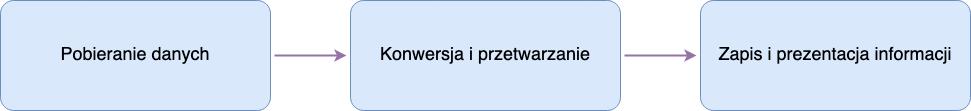
\includegraphics[width=0.8\textwidth]{img/scraping-process}
    \caption{Proces Web Scrapingu}
    \label{fig:scraping-process}
\end{figure}

\subsubsection{Pobieranie danych}

Pierwszy etapem procesu jest pobranie danych zawierających interesujące nas treści.
Zazwyczaj realizuje się to poprzez wysłanie zapytań HTTP (ang. \emph{Hypertext Transfer Protocol}) do jednego lub wielu serwerów WWW\@.
Pobrane, surowe dane zwykle są w formacie HTML (ang. \emph{Hypertext Markup Language}), XML (ang. \emph{Extensible Markup Language}) lub JSON (ang. \emph{JavaScript Object Notation}).

To kluczowy etap z perspektywy cyberbezpieczeństwa, ponieważ to właśnie w nim scraper wchodzi w bezpośrednią interakcję z scrapowaną infrastrukturą.
W związku z zabezpieczeniami stosowanymi przez serwery, ich dostępnością, wydajnością oraz ograniczeniami sieciowymi, etap ten jest zwykle najdłuższym w całym procesie.

\subsubsection{Konwersja i przetwarzanie}

Drugi etap procesu, konwersja i przetwarzanie, obejmuje operacje przekształcenia wcześniej pobranych danych, takie jak:
\begin{enumerate}
    \item Parsowanie - przekształcenie danych w strukturalną reprezentację łatwiejszą do dalszego przetwarzania
    \item Ekstrakcja - wyodrębnienie interesujących treści
    \item Filtracja - usunięcie niepożądanych i błędnych danych
    \item Mapowanie - przekształcenie danych do pożądanego, jednolitego formatu
\end{enumerate}

\noindent W przypadku scrapowania danych z wielu różnych źródeł, kluczowe jest ich dopasowanie do jednego wspólnego interfejsu, co ułatwia połączenie ich w spójny zbiór danych.

\subsubsection{Zapis i prezentacja informacji}

Ostatni etap Web Scrapingu, obejmujący zapis i prezentację informacji, odgrywa kluczową rolę w udostępnianiu zebranych danych użytkownikom końcowym w przystępnej i zrozumiałej formie\cite{iee-state-of-the-art}.

Dane mogą zostać zapisane w różny sposób, w zależności od potrzeb i preferencji użytkowników docelowych.
Najczęściej stosuje się bazy danych, pliki tekstowe lub arkusze kalkulacyjne, takie jak CSV (ang. \emph{Comma-Separated Values}) czy XLSX (ang. \emph{Microsoft Excel Open XML Spreadsheet}).
Kluczowe jest, aby dane były zapisywane w formatach umożliwiających łatwą przetwarzalność i analizę, co znacznie ułatwia ich dalsze wykorzystanie i analizę\cite{iee-state-of-the-art}.

Prezentacja danych to proces konwersji zebranych informacji na formę wizualną lub tekstową, dostosowaną do łatwego zrozumienia i interpretacji przez użytkowników.
Ten krok może obejmować tworzenie wykresów, tabel, raportów, interfejsów użytkownika oraz innych form wizualizacji, które umożliwiają szybką analizę i wnioskowanie na podstawie dostępnych danych.
Celem jest przedstawienie informacji w klarowny, przystępny sposób, który odpowiada na pytania odbiorców.

\subsection{Metody Web Scrapingu}\label{subsec:web-scraping-methods}

\subsubsection{Kopiuj-Wklej}

\subsubsection{Z wykorzystaniem przeglądarki internetowej}

\subsubsection{Za pomocą żądań HTTP}
